\section{
آشنایی با تراشه 74181
}

در این بخش با استفاده از تراشه
74181
و مطابق شکل
\eqref{fig:circuit1}
یک
ALU
با دو ورودی
A
و
B
می‌سازیم که دارای یک کنترل‌کننده است.
به طوری که با دادن کدهای مختلف به
،ALU
اعمال مختلف بر روی ورودی‌ها انجام می‌شود.

\begin{figure}[h!]
    \centering
    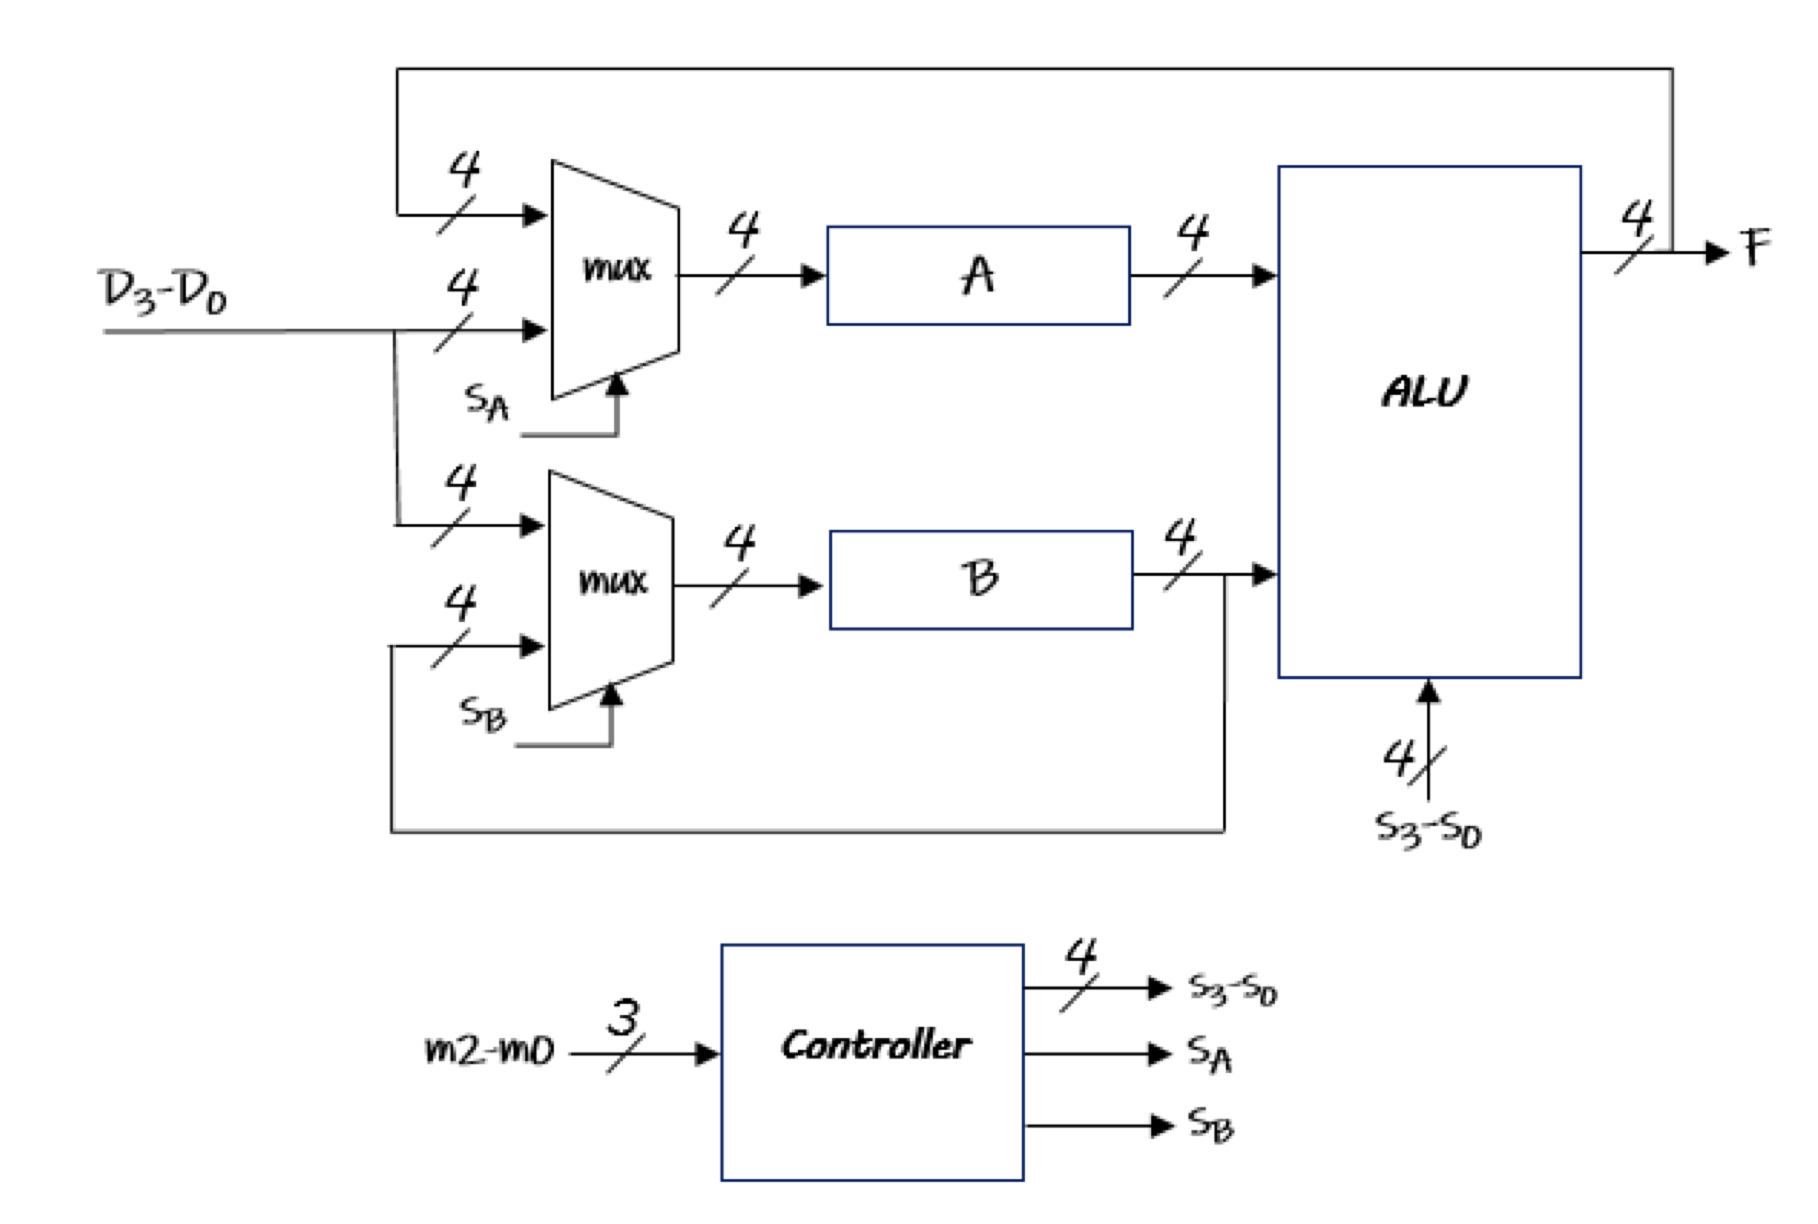
\includegraphics[width=0.9\textwidth]{part1/circuit.png}
    \caption{
    مدار بخش اول
    }
    \label{fig:circuit1}
\end{figure}

\subsection{
سیگنال‌های ورودی
}
\begin{enumerate}
    \item خطوط داده
    \lr{D0-D3}
    \item خطوط دستور
    \lr{M0-M2}
    \item یک کلید از نوع
    push-button
    برای باز گرداندن مدار به حالت اولیه
    (Reset)
    \item یک کلید از نوع
    push-button
    برای ورودی
    clock
\end{enumerate}

\subsection{
سیگنال‌های خروجی
}
\begin{enumerate}
    \item محتویات ثبات‌های
    A و B
    \item خروجی ALU
\end{enumerate}

\subsection{
طرز کار
}
برای ساخت مدار از تراشه‌های
\lr{74181 (ALU)}،
\lr{74175 (Registers)}،
\lr{74157 (MUX)}،
و تعداد کافی گیت پایه استفاده می‌کنیم.

\begin{figure}[h!]
    \centering
    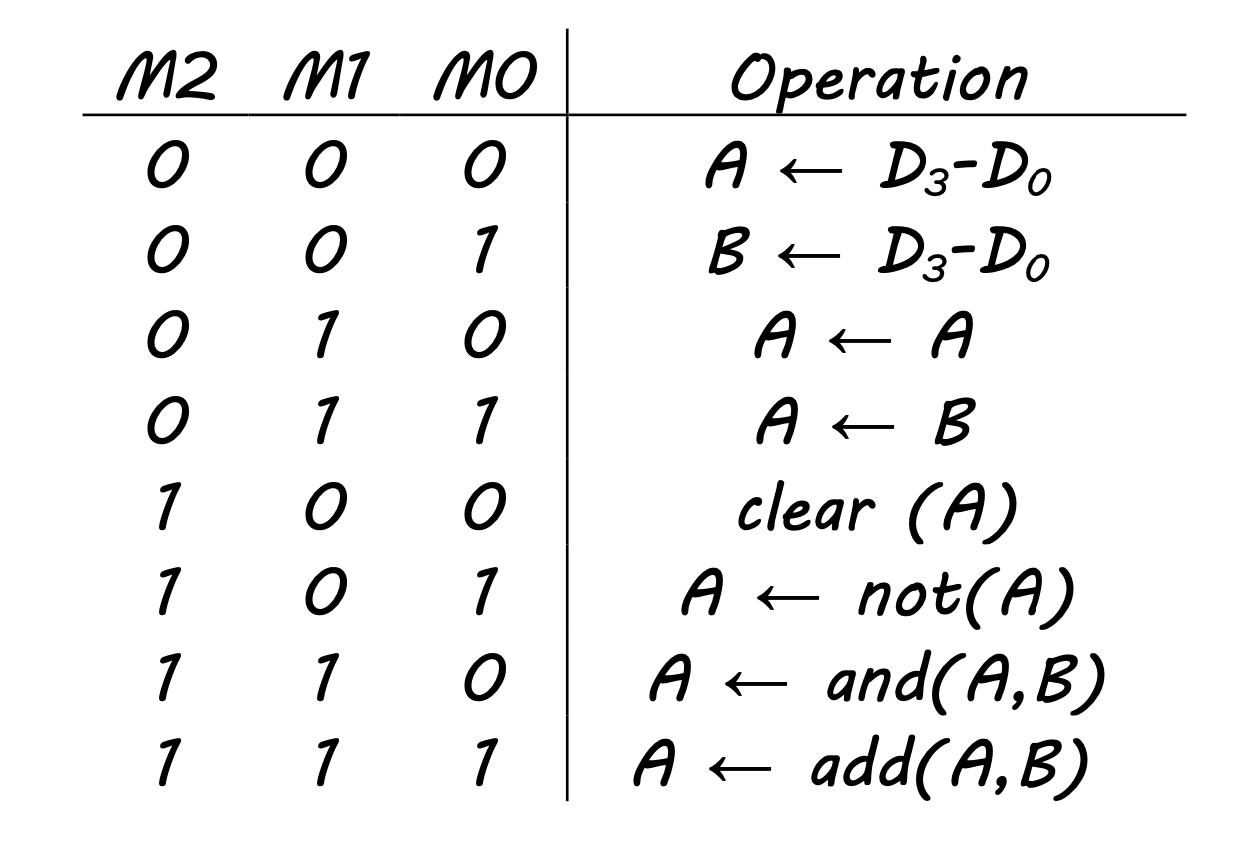
\includegraphics[width=0.5\textwidth]{part1/table.png}
    \caption{
    عملیات صورت گرفته بر حسب ورودی‌های کنترلی
    }
    \label{fig:table}
\end{figure}

در صفحه‌ی بعد ساده‌سازی و جدول ورودی‌های تراشه‌های به کار رفته آورده شده است.
از آنجایی که مدار با این گیت‌ها کمی شلوغ می‌شده در مدار نهایی به جای استفاده از گیت‌ها از یک دیکدر استفاده شده.
شکل مدار نهایی این بخش نیز در ادامه آمده است.
مدار به دو صورت
\lr{Active-High}
و
\lr{Active-Low}
بسته شده است.
همچنین جدول عملکرد تراشه‌ی ۷۴۱۸۱ که جدول‌ها مطابق آن بدست آمده در
شکل
\eqref{fig:table}
آمده است.

\begin{figure}[h!]
    \centering
    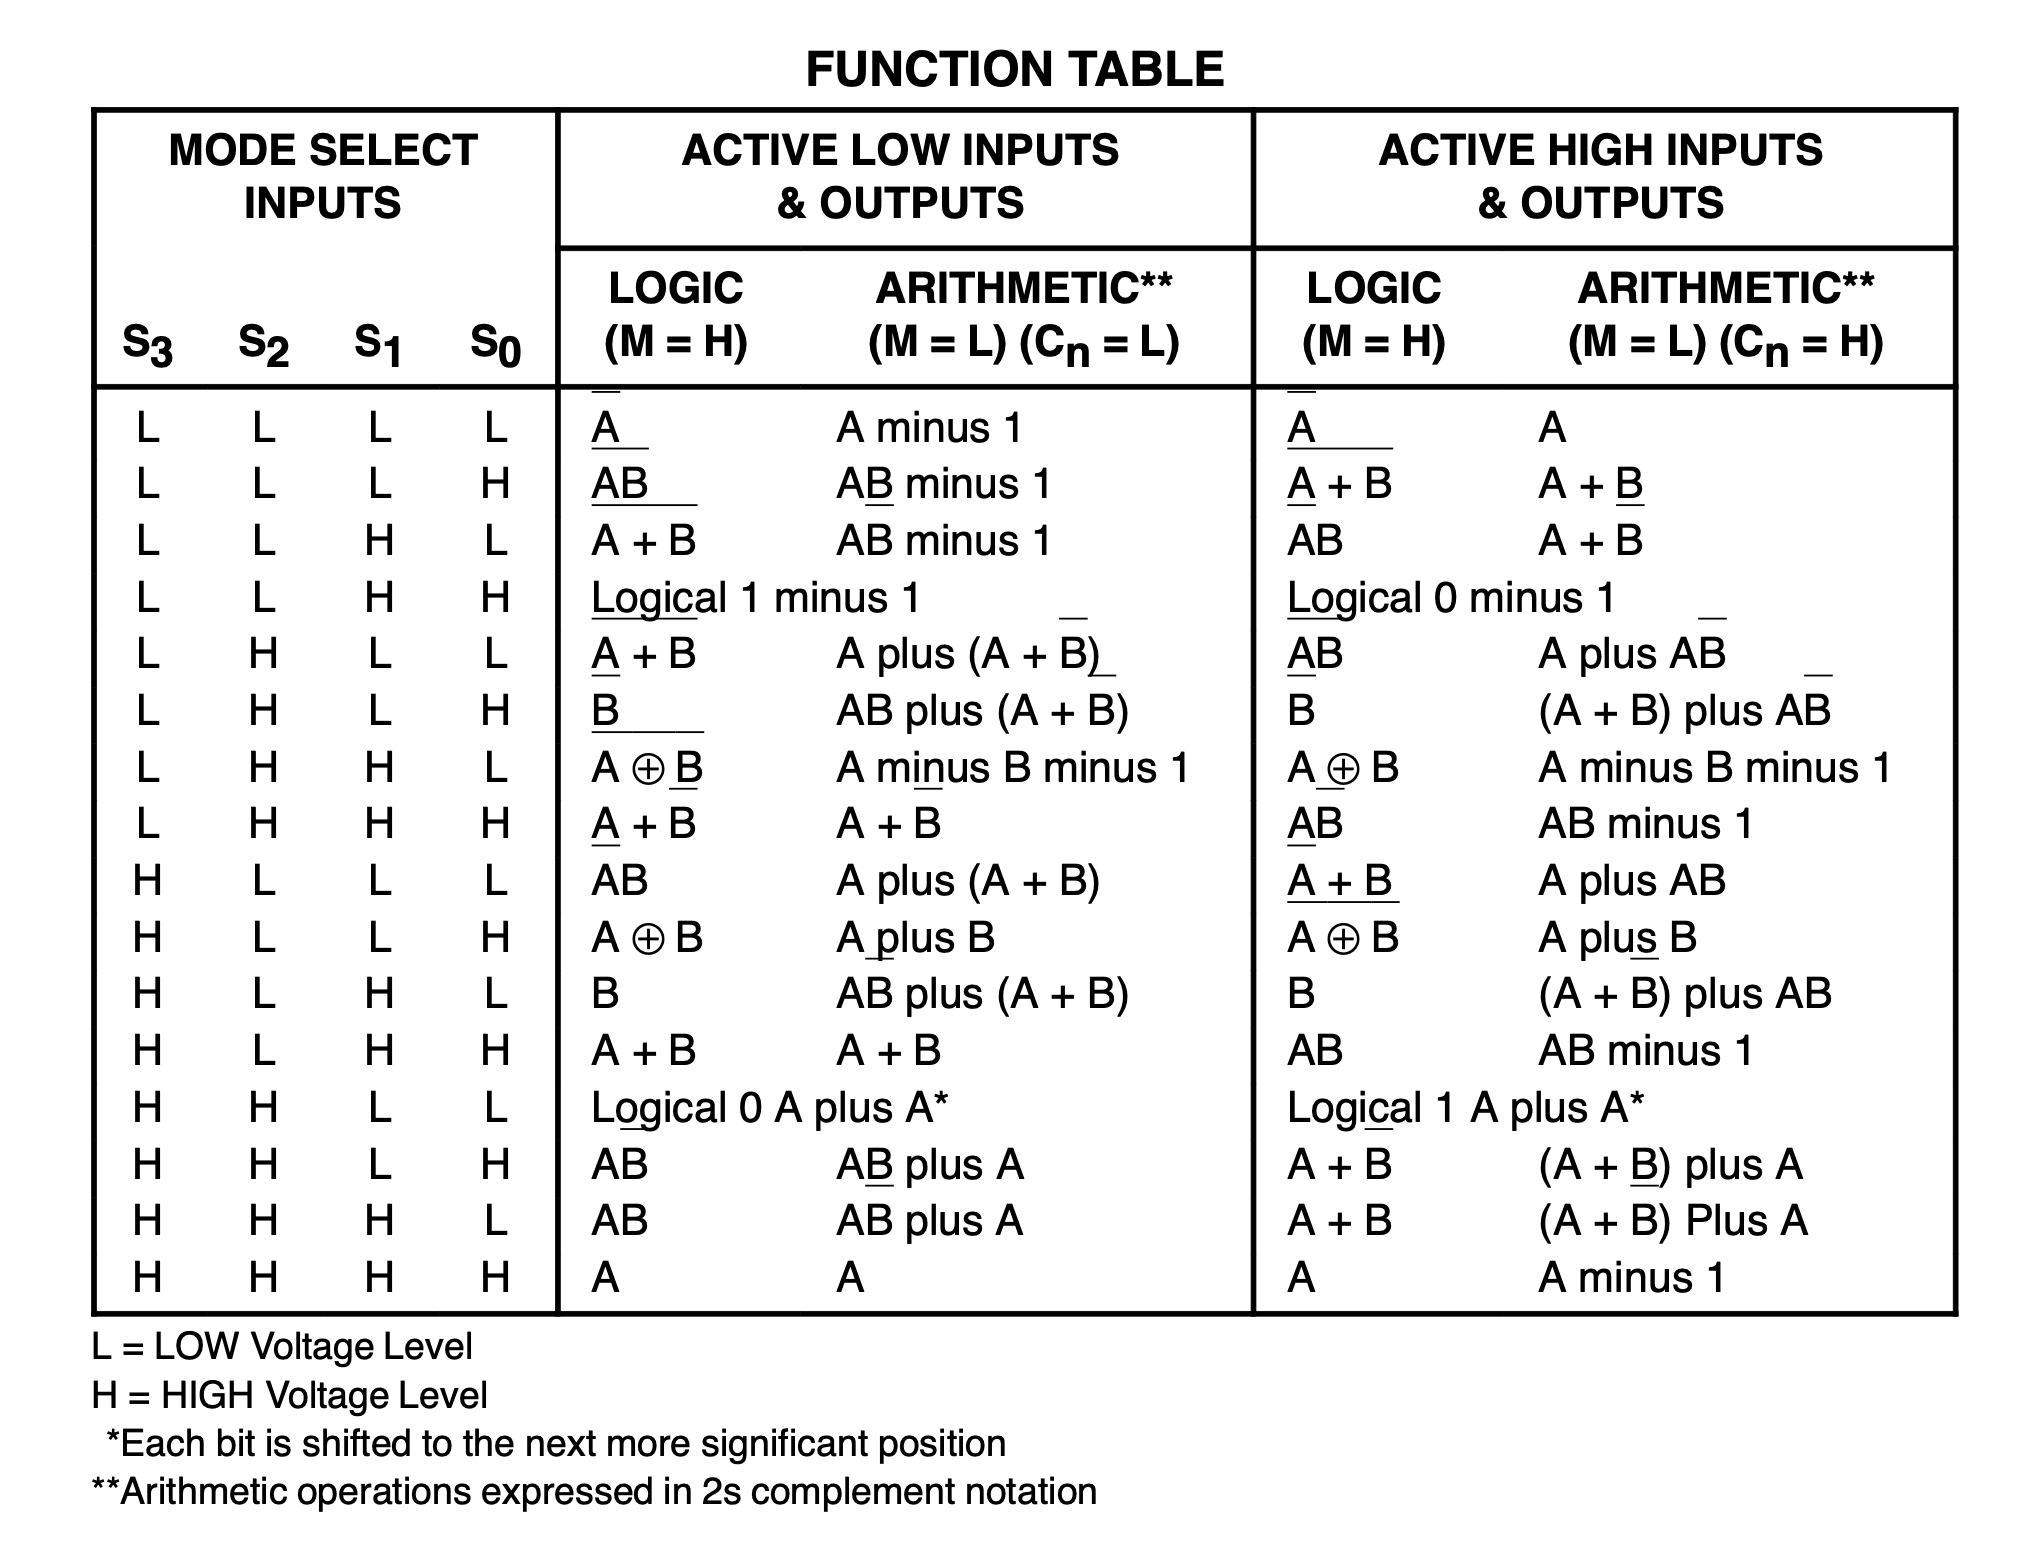
\includegraphics[width=\textwidth]{part1/datasheet.png}
    \caption{
    جدول عملکرد پردازنده
    ALU
    74181
    }
    \label{fig:table}
\end{figure}

\begin{figure}[h!]
    \centering
    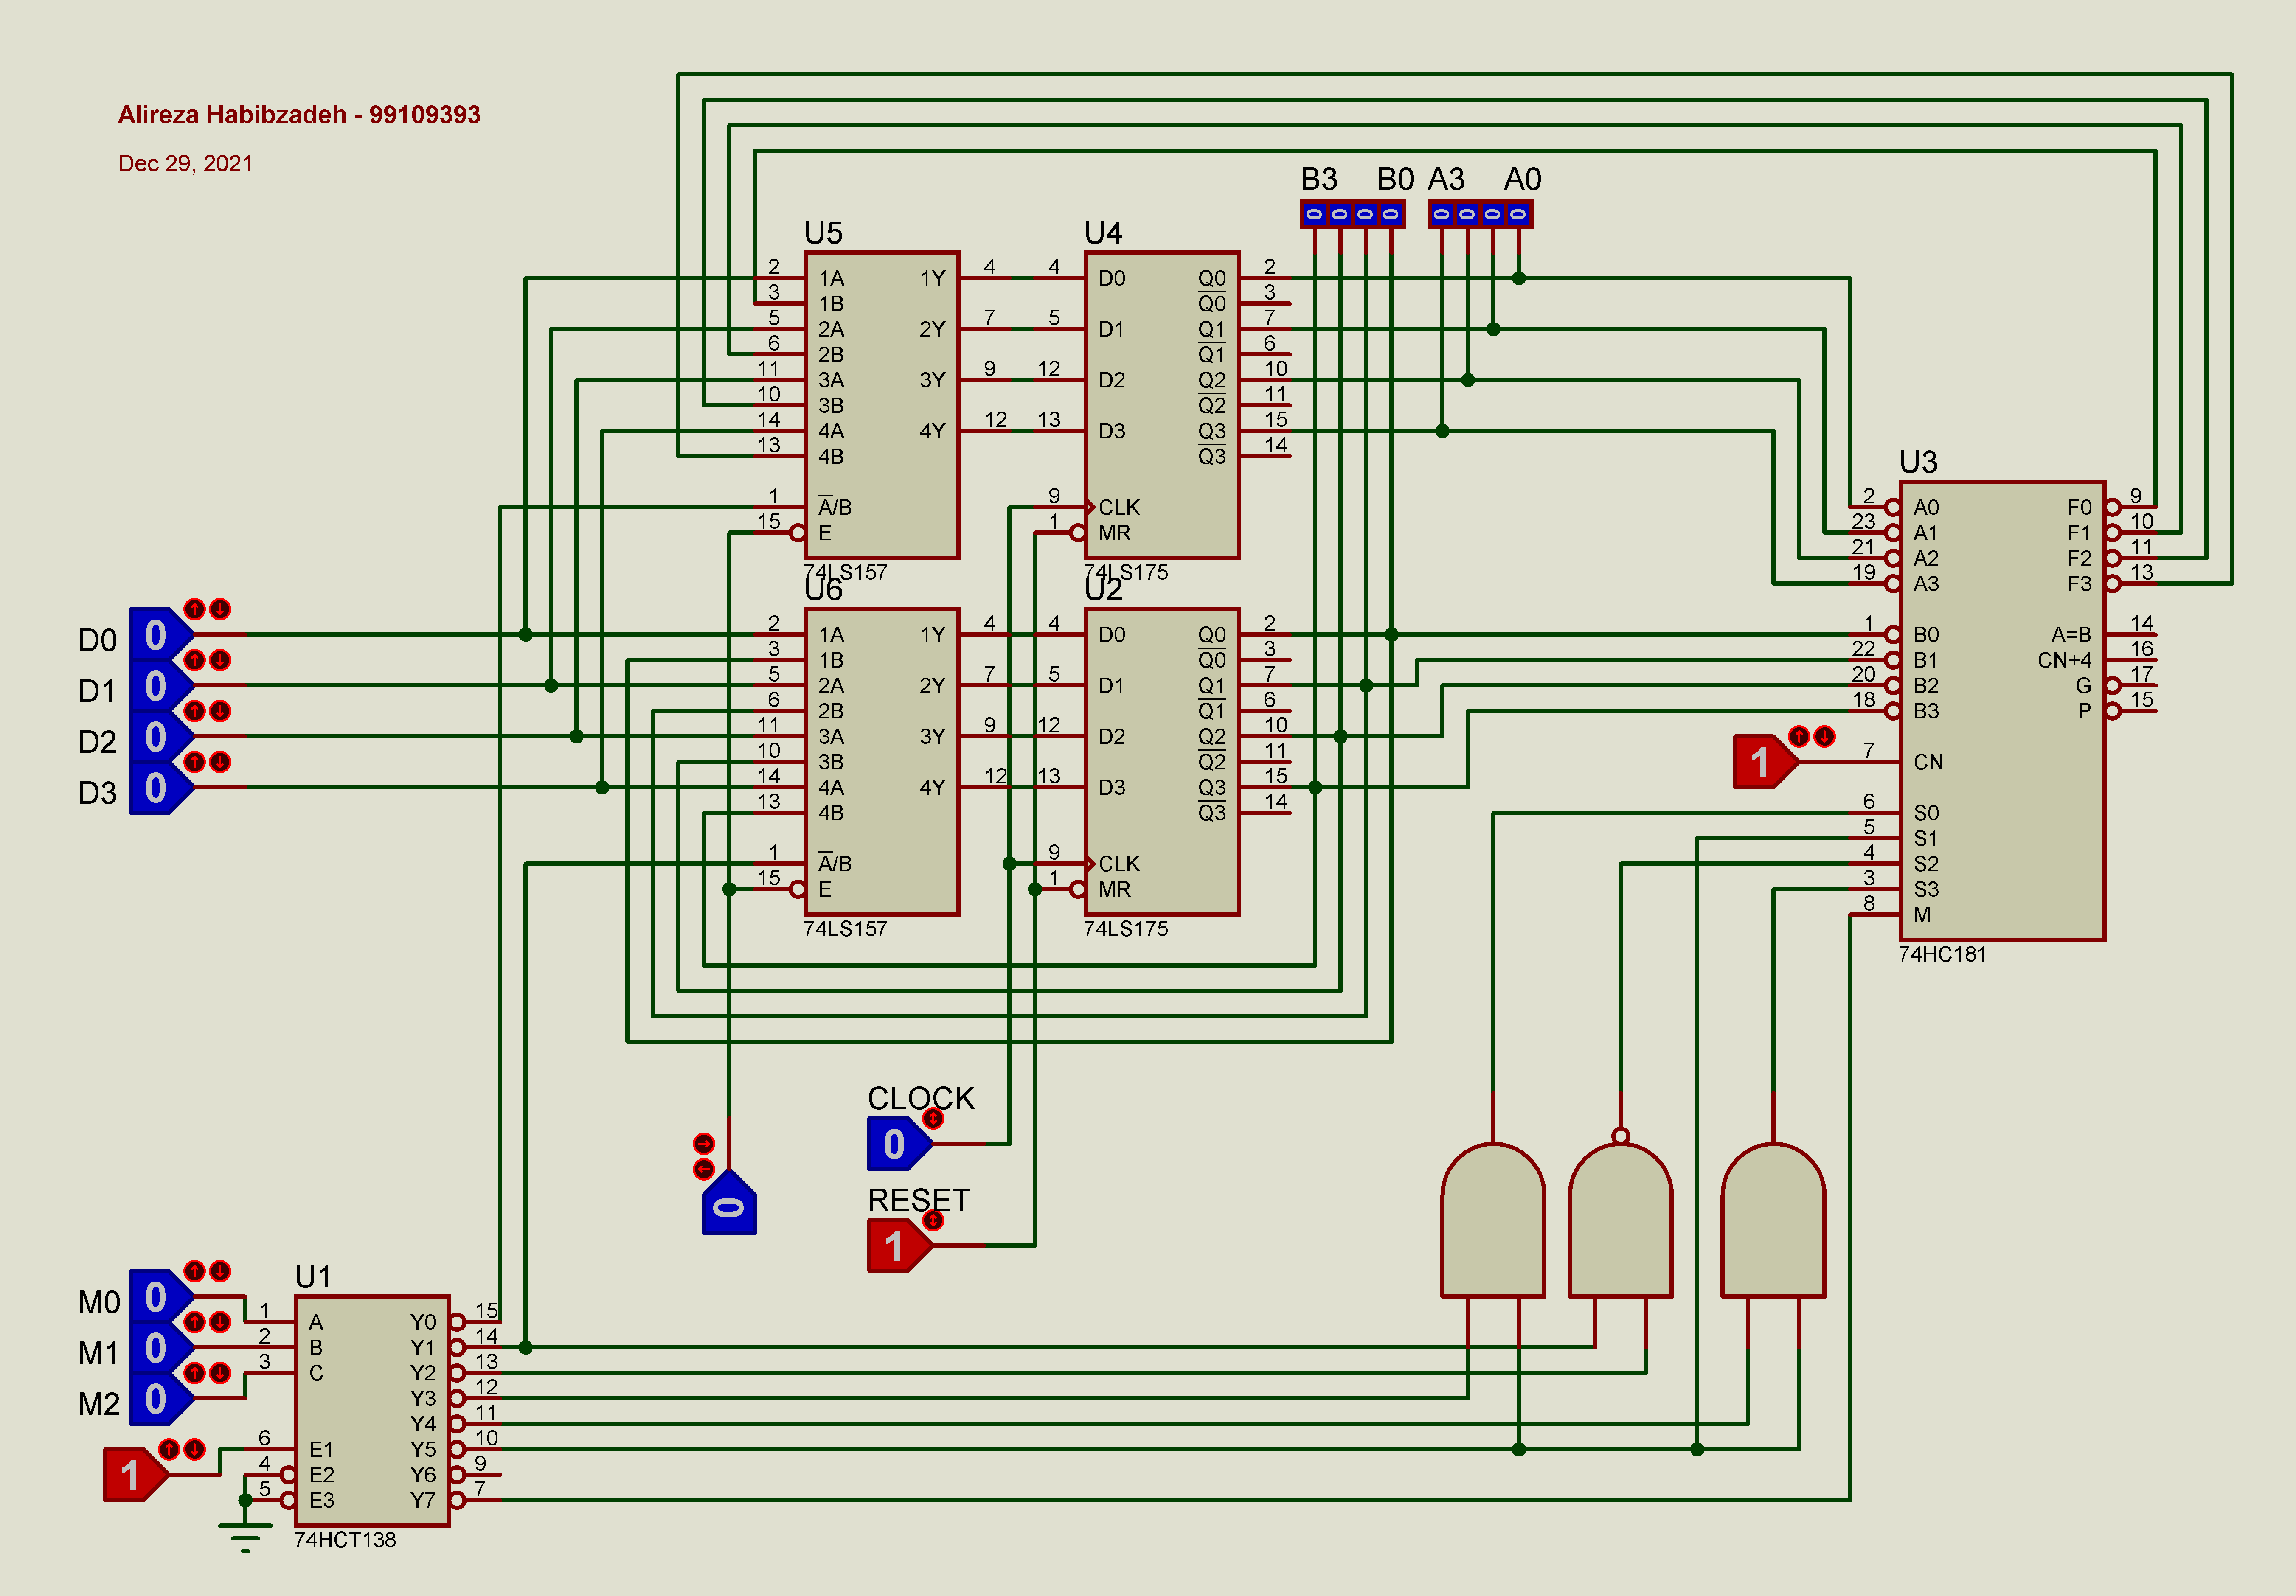
\includegraphics[width=\textwidth]{part1/74181.png}
    \caption{
    مدار
    \lr{Active-High}
    }
\end{figure}

\begin{figure}[h!]
    \centering
    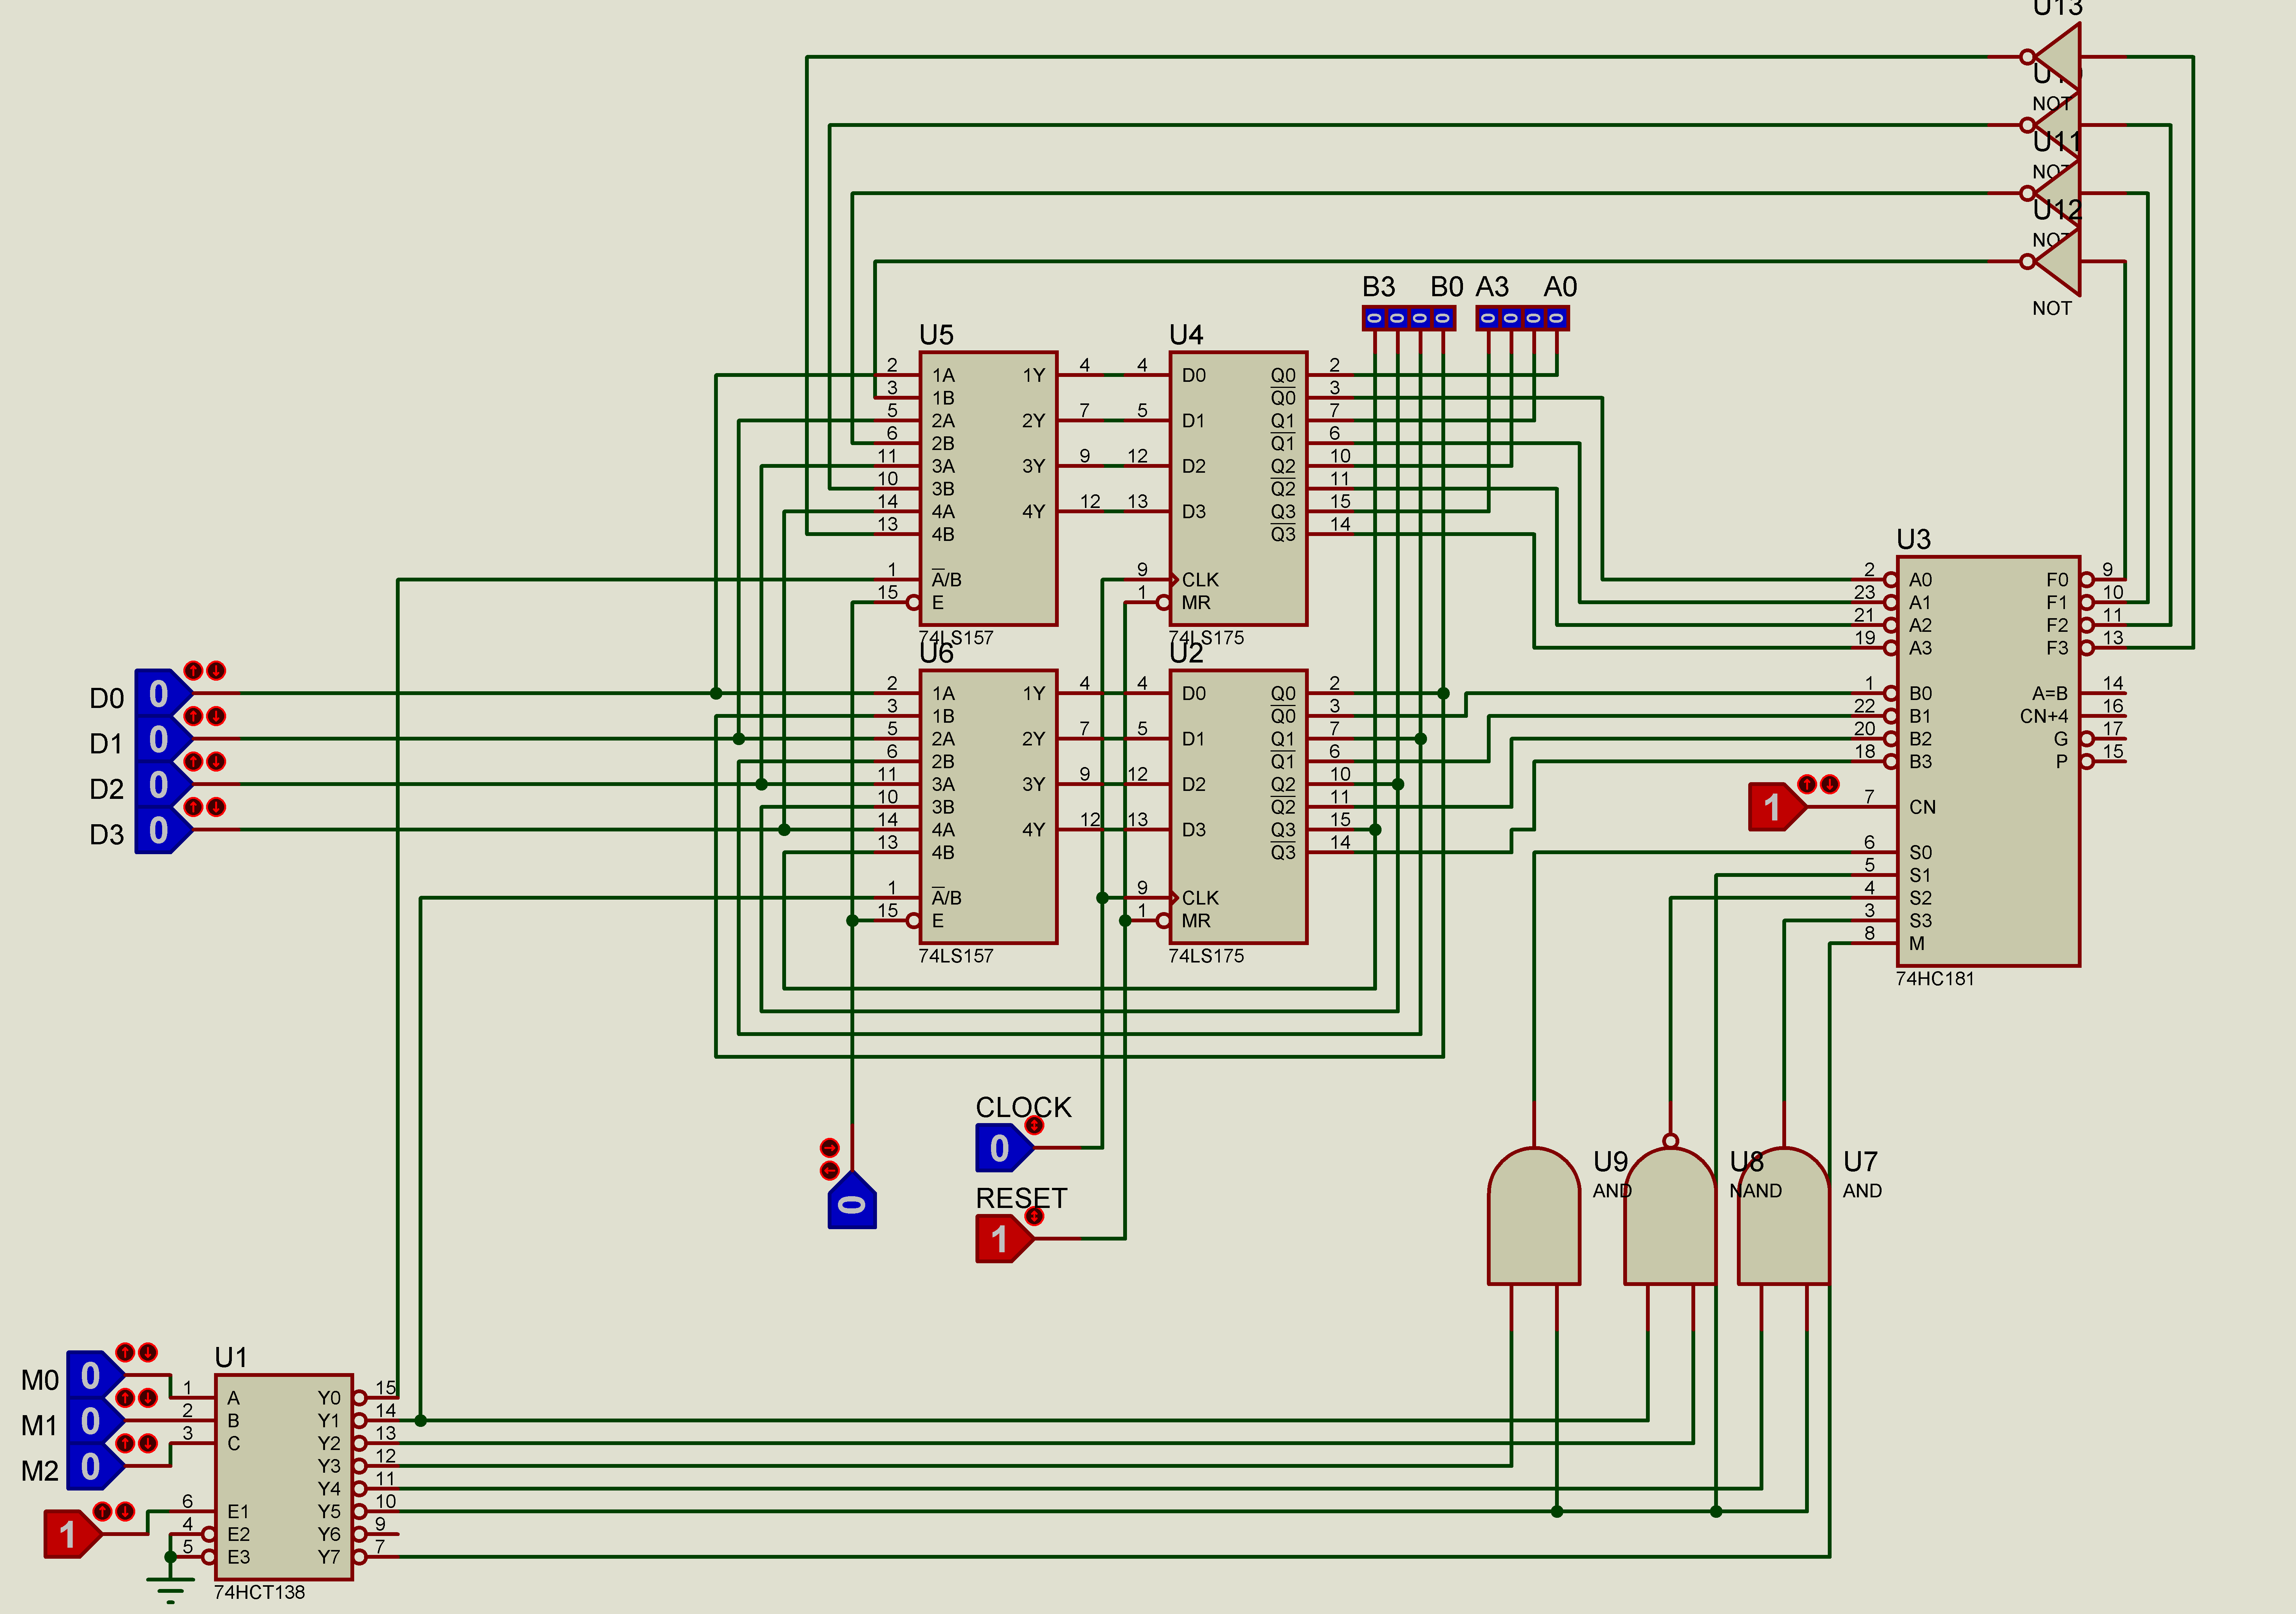
\includegraphics[width=\textwidth]{part1/74181-ActiveLow.png}
    \caption{
    مدار
    \lr{Active-Low}
    }
\end{figure}

\newpage